\documentclass[]{article}
\usepackage{lmodern}
\usepackage{amssymb,amsmath}
\usepackage{ifxetex,ifluatex}
\usepackage{fixltx2e} % provides \textsubscript
\ifnum 0\ifxetex 1\fi\ifluatex 1\fi=0 % if pdftex
  \usepackage[T1]{fontenc}
  \usepackage[utf8]{inputenc}
\else % if luatex or xelatex
  \ifxetex
    \usepackage{mathspec}
  \else
    \usepackage{fontspec}
  \fi
  \defaultfontfeatures{Ligatures=TeX,Scale=MatchLowercase}
\fi
% use upquote if available, for straight quotes in verbatim environments
\IfFileExists{upquote.sty}{\usepackage{upquote}}{}
% use microtype if available
\IfFileExists{microtype.sty}{%
\usepackage{microtype}
\UseMicrotypeSet[protrusion]{basicmath} % disable protrusion for tt fonts
}{}
\usepackage[margin=1in]{geometry}
\usepackage{hyperref}
\hypersetup{unicode=true,
            pdftitle={Forecasting Australian GDP},
            pdfborder={0 0 0},
            breaklinks=true}
\urlstyle{same}  % don't use monospace font for urls
\usepackage{graphicx,grffile}
\makeatletter
\def\maxwidth{\ifdim\Gin@nat@width>\linewidth\linewidth\else\Gin@nat@width\fi}
\def\maxheight{\ifdim\Gin@nat@height>\textheight\textheight\else\Gin@nat@height\fi}
\makeatother
% Scale images if necessary, so that they will not overflow the page
% margins by default, and it is still possible to overwrite the defaults
% using explicit options in \includegraphics[width, height, ...]{}
\setkeys{Gin}{width=\maxwidth,height=\maxheight,keepaspectratio}
\IfFileExists{parskip.sty}{%
\usepackage{parskip}
}{% else
\setlength{\parindent}{0pt}
\setlength{\parskip}{6pt plus 2pt minus 1pt}
}
\setlength{\emergencystretch}{3em}  % prevent overfull lines
\providecommand{\tightlist}{%
  \setlength{\itemsep}{0pt}\setlength{\parskip}{0pt}}
\setcounter{secnumdepth}{0}
% Redefines (sub)paragraphs to behave more like sections
\ifx\paragraph\undefined\else
\let\oldparagraph\paragraph
\renewcommand{\paragraph}[1]{\oldparagraph{#1}\mbox{}}
\fi
\ifx\subparagraph\undefined\else
\let\oldsubparagraph\subparagraph
\renewcommand{\subparagraph}[1]{\oldsubparagraph{#1}\mbox{}}
\fi

%%% Use protect on footnotes to avoid problems with footnotes in titles
\let\rmarkdownfootnote\footnote%
\def\footnote{\protect\rmarkdownfootnote}

%%% Change title format to be more compact
\usepackage{titling}

% Create subtitle command for use in maketitle
\newcommand{\subtitle}[1]{
  \posttitle{
    \begin{center}\large#1\end{center}
    }
}

\setlength{\droptitle}{-2em}
  \title{Forecasting Australian GDP}
  \pretitle{\vspace{\droptitle}\centering\huge}
  \posttitle{\par}
  \author{}
  \preauthor{}\postauthor{}
  \date{}
  \predate{}\postdate{}

\usepackage{booktabs}
\usepackage{longtable}
\usepackage{array}
\usepackage{multirow}
\usepackage[table]{xcolor}
\usepackage{wrapfig}
\usepackage{float}
\usepackage{colortbl}
\usepackage{pdflscape}
\usepackage{tabu}
\usepackage{threeparttable}
\usepackage{threeparttablex}
\usepackage[normalem]{ulem}
\usepackage{makecell}

\begin{document}
\maketitle

\section{Income Approach - Point
forecasting}\label{income-approach---point-forecasting}

\subsection{Summary of GDP - The most aggregate
series}\label{summary-of-gdp---the-most-aggregate-series}

\begin{table}[H]
\centering
\begin{tabular}{l|r|r|r|r|r|r|r|r|r|r|r|r|r|r|r|r}
\hline
\multicolumn{1}{c|}{ } & \multicolumn{8}{|c|}{ETS} & \multicolumn{8}{|c}{ARIMA} \\
\cline{2-9} \cline{10-17}
\multicolumn{1}{c|}{ } & \multicolumn{4}{|c|}{MSE} & \multicolumn{4}{|c|}{MASE} & \multicolumn{4}{|c|}{MSE} & \multicolumn{4}{|c}{MASE} \\
\cline{2-5} \cline{6-9} \cline{10-13} \cline{14-17}
Method & 1 & 2 & 3 & 4 & 1 & 2 & 3 & 4 & 1 & 2 & 3 & 4 & 1 & 2 & 3 & 4\\
\hline
Benchmark & -418.74 & -135.45 & -36.30 & -3.10 & -127.28 & -69.39 & -28.70 & -21.03 & -420.06 & -128.25 & -39.11 & -15.49 & -140.89 & -67.24 & -38.84 & -28.69\\
\hline
Base & 0.00 & 0.00 & 0.00 & 0.00 & 0.00 & 0.00 & 0.00 & 0.00 & 0.00 & 0.00 & 0.00 & 0.00 & 0.00 & 0.00 & 0.00 & 0.00\\
\hline
Bottom-up & -17.93 & -3.68 & 7.80 & 9.35 & -5.62 & -3.49 & -4.36 & -15.49 & -9.15 & 7.01 & 10.74 & 13.18 & -13.13 & -1.12 & -6.25 & -9.78\\
\hline
OLS & -0.18 & 3.45 & 6.05 & 6.70 & 0.05 & 0.96 & 3.47 & 1.50 & 2.12 & 2.46 & 2.54 & 1.92 & -0.83 & 1.84 & 0.75 & 0.62\\
\hline
WLS & -4.05 & 5.59 & 11.57 & 13.09 & -0.67 & 2.96 & 3.32 & -2.27 & 2.41 & 6.80 & 9.35 & 9.71 & -4.14 & 1.41 & 1.05 & -1.78\\
\hline
MinT Shrink & -0.72 & 5.86 & 9.33 & 9.70 & 3.25 & 5.14 & 4.63 & -1.15 & 7.06 & 9.05 & 8.63 & 9.73 & -0.14 & 0.93 & 1.23 & 0.39\\
\hline
\end{tabular}
\end{table}

\subsubsection{Summary of all aggregate level
series}\label{summary-of-all-aggregate-level-series}

\begin{table}[H]
\centering
\begin{tabular}{l|r|r|r|r|r|r|r|r|r|r|r|r|r|r|r|r}
\hline
\multicolumn{1}{c|}{ } & \multicolumn{8}{|c|}{ETS} & \multicolumn{8}{|c}{ARIMA} \\
\cline{2-9} \cline{10-17}
\multicolumn{1}{c|}{ } & \multicolumn{4}{|c|}{MSE} & \multicolumn{4}{|c|}{MASE} & \multicolumn{4}{|c|}{MSE} & \multicolumn{4}{|c}{MASE} \\
\cline{2-5} \cline{6-9} \cline{10-13} \cline{14-17}
Method & 1 & 2 & 3 & 4 & 1 & 2 & 3 & 4 & 1 & 2 & 3 & 4 & 1 & 2 & 3 & 4\\
\hline
Benchmark & -320.17 & -101.63 & -29.68 & -2.32 & -96 & -40.28 & -11.83 & -1.92 & -298.21 & -86.44 & -19.78 & 0.71 & -78.18 & -36.49 & -11.83 & -2.91\\
\hline
Base & 0.00 & 0.00 & 0.00 & 0.00 & 0 & 0.00 & 0.00 & 0.00 & 0.00 & 0.00 & 0.00 & 0.00 & 0.00 & 0.00 & 0.00 & 0.00\\
\hline
Bottom-up & -7.64 & -2.49 & 0.73 & 1.55 & -2 & 0.00 & -2.15 & -1.92 & 1.61 & 8.32 & 5.18 & 9.05 & 1.82 & 1.35 & -1.08 & 0.00\\
\hline
OLS & 3.16 & 3.29 & 2.91 & 2.92 & 2 & 2.78 & 2.15 & 1.92 & 4.79 & 4.33 & 3.05 & 3.37 & 1.82 & 1.35 & 1.08 & 1.94\\
\hline
WLS & 3.61 & 4.84 & 4.39 & 4.45 & 4 & 4.17 & 2.15 & 1.92 & 7.89 & 8.49 & 6.94 & 8.15 & 3.64 & 2.70 & 1.08 & 1.94\\
\hline
MinT Shrink & 6.46 & 5.18 & 2.39 & 1.54 & 6 & 4.17 & 3.23 & 2.88 & 12.69 & 11.96 & 6.76 & 8.69 & 7.27 & 5.41 & 2.15 & 4.85\\
\hline
\end{tabular}
\end{table}

\subsection{Summary of all disaggregate
series}\label{summary-of-all-disaggregate-series}

\begin{table}[H]
\centering
\begin{tabular}{l|r|r|r|r|r|r|r|r|r|r|r|r|r|r|r|r}
\hline
\multicolumn{1}{c|}{ } & \multicolumn{8}{|c|}{ETS} & \multicolumn{8}{|c}{ARIMA} \\
\cline{2-9} \cline{10-17}
\multicolumn{1}{c|}{ } & \multicolumn{4}{|c|}{MSE} & \multicolumn{4}{|c|}{MASE} & \multicolumn{4}{|c|}{MSE} & \multicolumn{4}{|c}{MASE} \\
\cline{2-5} \cline{6-9} \cline{10-13} \cline{14-17}
Method & 1 & 2 & 3 & 4 & 1 & 2 & 3 & 4 & 1 & 2 & 3 & 4 & 1 & 2 & 3 & 4\\
\hline
Benchmark & -200.06 & -71.72 & -21.93 & -0.40 & -61.02 & -30.67 & -11.11 & -2.02 & -191.76 & -64.02 & -7.71 & 6.65 & -63.79 & -32.43 & -13.64 & -4.12\\
\hline
Base & 0.00 & 0.00 & 0.00 & 0.00 & 0.00 & 0.00 & 0.00 & 0.00 & 0.00 & 0.00 & 0.00 & 0.00 & 0.00 & 0.00 & 0.00 & 0.00\\
\hline
Bottom-up & 0.00 & 0.00 & 0.00 & 0.00 & 0.00 & 0.00 & 0.00 & 0.00 & 0.00 & 0.00 & 0.00 & 0.00 & 0.00 & 0.00 & 0.00 & 0.00\\
\hline
OLS & 0.66 & -2.57 & -3.50 & -3.73 & -23.73 & -26.67 & -18.89 & -12.12 & -2.88 & -5.33 & -2.55 & -4.91 & -20.69 & -24.32 & -22.73 & -20.62\\
\hline
WLS & 6.18 & 3.62 & 1.38 & 0.28 & 1.69 & 0.00 & -1.11 & 0.00 & 2.43 & -0.25 & 2.93 & 0.29 & 0.00 & -1.35 & -1.14 & 0.00\\
\hline
MinT Shrink & 8.78 & 4.34 & 0.58 & -1.43 & 3.39 & 1.33 & 1.11 & 1.01 & 4.81 & 1.57 & 2.15 & 0.47 & 0.00 & -1.35 & -1.14 & 0.00\\
\hline
\end{tabular}
\end{table}

\subsection{Summary of all series in the hierarchy (Average over all
series)}\label{summary-of-all-series-in-the-hierarchy-average-over-all-series}

\begin{table}[H]
\centering
\begin{tabular}{l|r|r|r|r|r|r|r|r|r|r|r|r|r|r|r|r}
\hline
\multicolumn{1}{c|}{ } & \multicolumn{8}{|c|}{ETS} & \multicolumn{8}{|c}{ARIMA} \\
\cline{2-9} \cline{10-17}
\multicolumn{1}{c|}{ } & \multicolumn{4}{|c|}{MSE} & \multicolumn{4}{|c|}{MASE} & \multicolumn{4}{|c|}{MSE} & \multicolumn{4}{|c}{MASE} \\
\cline{2-5} \cline{6-9} \cline{10-13} \cline{14-17}
Method & 1 & 2 & 3 & 4 & 1 & 2 & 3 & 4 & 1 & 2 & 3 & 4 & 1 & 2 & 3 & 4\\
\hline
Benchmark & -295.40 & -96.29 & -28.41 & -2.01 & -71.43 & -33.78 & -10.99 & -1.98 & -276.70 & -82.54 & -17.73 & 1.68 & -68.42 & -33.78 & -12.22 & -4.04\\
\hline
Base & 0.00 & 0.00 & 0.00 & 0.00 & 0.00 & 0.00 & 0.00 & 0.00 & 0.00 & 0.00 & 0.00 & 0.00 & 0.00 & 0.00 & 0.00 & 0.00\\
\hline
Bottom-up & -6.06 & -2.05 & 0.61 & 1.31 & 0.00 & 0.00 & -1.10 & 0.00 & 1.28 & 6.88 & 4.30 & 7.57 & 1.75 & 0.00 & 0.00 & 0.00\\
\hline
OLS & 2.64 & 2.24 & 1.86 & 1.87 & -14.29 & -14.86 & -10.99 & -6.93 & 3.24 & 2.65 & 2.09 & 2.01 & -12.28 & -14.86 & -13.33 & -12.12\\
\hline
WLS & 4.14 & 4.62 & 3.89 & 3.79 & 3.57 & 1.35 & 0.00 & 0.99 & 6.79 & 6.97 & 6.25 & 6.86 & 1.75 & 0.00 & 0.00 & 1.01\\
\hline
MinT Shrink & 6.94 & 5.03 & 2.09 & 1.07 & 5.36 & 2.70 & 2.20 & 1.98 & 11.10 & 10.15 & 5.98 & 7.34 & 3.51 & 1.35 & 0.00 & 1.01\\
\hline
\end{tabular}
\end{table}

\section{Income approach - Probabilistic forecasting (Non-parametric
Bootstrap
approach)}\label{income-approach---probabilistic-forecasting-non-parametric-bootstrap-approach}

\subsection{Predictive ability of multivariate forecast distribution of
the whole
hierarchy}\label{predictive-ability-of-multivariate-forecast-distribution-of-the-whole-hierarchy}

\begin{table}[H]
\centering
\begin{tabular}{l|r|r|r|r|r|r|r|r|r|r|r|r|r|r|r|r}
\hline
\multicolumn{1}{c|}{ } & \multicolumn{8}{|c|}{ETS} & \multicolumn{8}{|c}{ARIMA} \\
\cline{2-9} \cline{10-17}
\multicolumn{1}{c|}{ } & \multicolumn{4}{|c|}{ES} & \multicolumn{4}{|c|}{VS} & \multicolumn{4}{|c|}{ES} & \multicolumn{4}{|c}{VS} \\
\cline{2-5} \cline{6-9} \cline{10-13} \cline{14-17}
Method & 1 & 2 & 3 & 4 & 1 & 2 & 3 & 4 & 1 & 2 & 3 & 4 & 1 & 2 & 3 & 4\\
\hline
Benchmark & -103.31 & -39.64 & -8.52 & 3.84 & -164.35 & -52.47 & -9.68 & 6.05 & -95.27 & -36.15 & -5.41 & 4.93 & -150.24 & -41.37 & 0.33 & 14.06\\
\hline
Base & 0.00 & 0.00 & 0.00 & 0.00 & 0.00 & 0.00 & 0.00 & 0.00 & 0.00 & 0.00 & 0.00 & 0.00 & 0.00 & 0.00 & 0.00 & 0.00\\
\hline
Bottom-up & 0.44 & 1.11 & -0.99 & -2.29 & 1.38 & 3.24 & 2.69 & 2.65 & 2.21 & 3.09 & 0.98 & 1.26 & 4.13 & 6.66 & 3.67 & 5.20\\
\hline
OLS & 2.35 & 2.25 & 1.77 & 1.85 & 0.72 & -1.08 & -0.74 & -0.11 & 2.29 & 2.02 & 1.61 & 1.55 & -0.91 & -0.43 & -0.14 & -0.37\\
\hline
WLS & 4.63 & 4.69 & 2.90 & 2.03 & 7.26 & 5.43 & 3.72 & 2.66 & 4.35 & 4.59 & 3.51 & 3.55 & 6.52 & 6.76 & 6.01 & 5.61\\
\hline
MinT Sample & 5.52 & 0.75 & -1.62 & -2.32 & 8.63 & -1.24 & -8.06 & -13.44 & 0.20 & -3.64 & -5.26 & -1.72 & -0.49 & -0.43 & -6.76 & -4.58\\
\hline
MinT Shrink & 6.34 & 5.16 & 3.18 & 2.27 & 9.84 & 6.06 & 3.34 & 1.05 & 6.32 & 4.61 & 3.34 & 4.88 & 8.79 & 9.20 & 6.34 & 6.79\\
\hline
\end{tabular}
\end{table}

\subsection{Predictive ability of univariate forecast
distributions}\label{predictive-ability-of-univariate-forecast-distributions}

\subsubsection{Summary of GDP - The most aggregate
series}\label{summary-of-gdp---the-most-aggregate-series-1}

\begin{table}[H]
\centering
\begin{tabular}{l|r|r|r|r|r|r|r|r}
\hline
\multicolumn{1}{c|}{ } & \multicolumn{4}{|c|}{ETS (CRPS)} & \multicolumn{4}{|c}{ARIMA (CRPS)} \\
\cline{2-5} \cline{6-9}
Method & 1 & 2 & 3 & 4 & 1 & 2 & 3 & 4\\
\hline
Benchmark & -139.03 & -60.56 & -17.03 & -5.22 & -144.75 & -56.38 & -22.61 & -9.99\\
\hline
Base & 0.00 & 0.00 & 0.00 & 0.00 & 0.00 & 0.00 & 0.00 & 0.00\\
\hline
Bottom-up & -6.01 & -2.62 & -2.92 & -12.05 & -7.99 & 1.29 & -2.93 & -4.41\\
\hline
OLS & -0.13 & 1.60 & 3.20 & 1.62 & 0.59 & 1.55 & 0.67 & 0.36\\
\hline
WLS & -0.95 & 3.20 & 3.80 & -0.75 & -0.63 & 2.79 & 1.46 & 0.27\\
\hline
MinT Sample & 3.29 & 1.26 & -0.09 & -4.15 & -4.68 & -9.35 & -9.40 & -5.79\\
\hline
MinT Shrink & 1.61 & 4.31 & 3.91 & -0.74 & 1.28 & 1.43 & 1.04 & 1.28\\
\hline
\end{tabular}
\end{table}

\subsubsection{Summary of all aggregate level
series}\label{summary-of-all-aggregate-level-series-1}

\begin{table}[H]
\centering
\begin{tabular}{l|r|r|r|r|r|r|r|r}
\hline
\multicolumn{1}{c|}{ } & \multicolumn{4}{|c|}{ETS (CRPS)} & \multicolumn{4}{|c}{ARIMA (CRPS)} \\
\cline{2-5} \cline{6-9}
Method & 1 & 2 & 3 & 4 & 1 & 2 & 3 & 4\\
\hline
Benchmark & -116.05 & -44.38 & -8.96 & 3.46 & -104.93 & -41.23 & -8.22 & 3.04\\
\hline
Base & 0.00 & 0.00 & 0.00 & 0.00 & 0.00 & 0.00 & 0.00 & 0.00\\
\hline
OLS & 2.12 & 2.22 & 1.99 & 1.84 & 2.18 & 1.75 & 0.99 & 1.69\\
\hline
WLS & 3.28 & 3.20 & 1.68 & 0.71 & 3.22 & 2.75 & 1.30 & 2.20\\
\hline
MinT Sample & 4.02 & -1.54 & -2.53 & -3.34 & -0.69 & -5.80 & -7.97 & -3.03\\
\hline
MinT Shrink & 4.84 & 3.53 & 2.07 & 1.09 & 5.93 & 3.13 & 1.02 & 3.81\\
\hline
\end{tabular}
\end{table}

\subsubsection{Summary of all disaggregate
series}\label{summary-of-all-disaggregate-series-1}

\begin{table}[H]
\centering
\begin{tabular}{l|r|r|r|r|r|r|r|r}
\hline
\multicolumn{1}{c|}{ } & \multicolumn{4}{|c|}{ETS (CRPS)} & \multicolumn{4}{|c}{ARIMA (CRPS)} \\
\cline{2-5} \cline{6-9}
Method & 1 & 2 & 3 & 4 & 1 & 2 & 3 & 4\\
\hline
Benchmark & -81.67 & -32.82 & -6.70 & 3.68 & -78.46 & -31.91 & -6.22 & 3.38\\
\hline
Base & 0.00 & 0.00 & 0.00 & 0.00 & 0.00 & 0.00 & 0.00 & 0.00\\
\hline
OLS & -6.79 & -8.46 & -6.40 & -4.31 & -8.31 & -10.13 & -8.85 & -8.94\\
\hline
WLS & 1.91 & 1.17 & 0.80 & 0.74 & 0.05 & 0.17 & 0.68 & 0.65\\
\hline
MinT Sample & 1.32 & -2.31 & -1.66 & -3.82 & -5.67 & -7.72 & -8.88 & -6.51\\
\hline
MinT Shrink & 3.91 & 2.19 & 1.99 & 1.30 & 0.36 & -0.37 & -0.04 & 1.06\\
\hline
\end{tabular}
\end{table}

\subsubsection{Summary of all series in the
hierarchy}\label{summary-of-all-series-in-the-hierarchy}

\begin{table}[H]
\centering
\begin{tabular}{l|r|r|r|r|r|r|r|r}
\hline
\multicolumn{1}{c|}{ } & \multicolumn{4}{|c|}{ETS (CRPS)} & \multicolumn{4}{|c}{ARIMA (CRPS)} \\
\cline{2-5} \cline{6-9}
Method & 1 & 2 & 3 & 4 & 1 & 2 & 3 & 4\\
\hline
Benchmark & -104.77 & -40.82 & -8.29 & 3.52 & -96.44 & -38.38 & -7.63 & 3.14\\
\hline
Base & 0.00 & 0.00 & 0.00 & 0.00 & 0.00 & 0.00 & 0.00 & 0.00\\
\hline
OLS & -0.81 & -1.07 & -0.48 & 0.05 & -1.18 & -1.88 & -1.91 & -1.40\\
\hline
WLS & 2.83 & 2.58 & 1.42 & 0.72 & 2.20 & 1.96 & 1.12 & 1.75\\
\hline
MinT Sample & 3.13 & -1.78 & -2.27 & -3.48 & -2.29 & -6.38 & -8.24 & -4.04\\
\hline
MinT Shrink & 4.53 & 3.11 & 2.05 & 1.15 & 4.14 & 2.06 & 0.71 & 3.01\\
\hline
\end{tabular}
\end{table}

\section{Income approach - Probabilistic forecasting (Parametric
approach assuming
Gaussianity)}\label{income-approach---probabilistic-forecasting-parametric-approach-assuming-gaussianity}

\subsection{Predictive ability in the multivariate forecast distribution
of the whole
hierarchy}\label{predictive-ability-in-the-multivariate-forecast-distribution-of-the-whole-hierarchy}

\begin{table}[H]
\centering
\begin{tabular}{l|r|r|r|r|r|r|r|r|r|r|r|r|r|r|r|r}
\hline
\multicolumn{1}{c|}{ } & \multicolumn{8}{|c|}{ETS} & \multicolumn{8}{|c}{ARIMA} \\
\cline{2-9} \cline{10-17}
\multicolumn{1}{c|}{ } & \multicolumn{4}{|c|}{ES} & \multicolumn{4}{|c|}{VS} & \multicolumn{4}{|c|}{ES} & \multicolumn{4}{|c}{VS} \\
\cline{2-5} \cline{6-9} \cline{10-13} \cline{14-17}
Method & 1 & 2 & 3 & 4 & 1 & 2 & 3 & 4 & 1 & 2 & 3 & 4 & 1 & 2 & 3 & 4\\
\hline
Benchmark & -96.14 & -36.28 & -6.59 & 5.26 & -156.30 & -50.32 & -9.15 & 6.00 & -88.32 & -32.30 & -3.07 & 6.61 & -145.36 & -40.81 & 0.21 & 13.59\\
\hline
Base & 0.00 & 0.00 & 0.00 & 0.00 & 0.00 & 0.00 & 0.00 & 0.00 & 0.00 & 0.00 & 0.00 & 0.00 & 0.00 & 0.00 & 0.00 & 0.00\\
\hline
Bottom-up & -0.09 & 0.84 & -1.11 & -2.53 & 1.08 & 2.99 & 2.51 & 2.44 & 2.24 & 3.06 & 0.81 & 1.09 & 4.11 & 6.63 & 3.45 & 4.93\\
\hline
OLS & 1.87 & 1.93 & 1.33 & 1.41 & 1.01 & -0.62 & -0.60 & 0.00 & 1.62 & 1.63 & 1.18 & 1.06 & -0.68 & -0.31 & 0.02 & -0.31\\
\hline
WLS & 3.85 & 4.00 & 2.05 & 1.16 & 7.41 & 5.61 & 3.62 & 2.64 & 3.51 & 3.77 & 2.62 & 2.68 & 6.31 & 6.69 & 5.86 & 5.54\\
\hline
MinT Sample & 4.58 & -0.14 & -2.41 & -2.78 & 8.48 & -1.36 & -8.09 & -13.39 & -0.44 & -4.27 & -5.78 & -2.11 & -0.65 & -0.55 & -6.82 & -4.65\\
\hline
MinT Shrink & 5.43 & 4.54 & 2.40 & 1.61 & 9.84 & 6.16 & 3.39 & 1.13 & 5.59 & 3.93 & 2.67 & 4.20 & 8.83 & 9.20 & 6.28 & 6.62\\
\hline
\end{tabular}
\end{table}

\begin{table}[H]
\centering
\begin{tabular}{l|r|r|r|r|r|r|r|r}
\hline
\multicolumn{1}{c|}{ } & \multicolumn{4}{|c|}{ETS} & \multicolumn{4}{|c}{ARIMA} \\
\cline{2-5} \cline{6-9}
Method & 1 & 2 & 3 & 4 & 1 & 2 & 3 & 4\\
\hline
Bottom-up & 0.0000 & 0.0000 & 0.0000 & 0.0000 & 0.0000 & 0.0000 & 0.0000 & 0.0000\\
\hline
OLS & -2.6202 & 5.6523 & 20.1662 & 34.2084 & -1.7115 & 7.2382 & 21.1612 & 34.3326\\
\hline
WLS & -0.2564 & -1.2158 & -1.6048 & -1.8090 & -0.4037 & -1.5222 & -1.6978 & -2.0367\\
\hline
MinT Sample & -3.4253 & -10.1779 & -15.7191 & -20.5008 & -4.9823 & -11.2533 & -15.9803 & -18.7421\\
\hline
MinT Shrink & -0.1630 & -1.5999 & -2.3983 & -2.9095 & -0.8188 & -2.3546 & -2.9066 & -3.3077\\
\hline
\end{tabular}
\end{table}

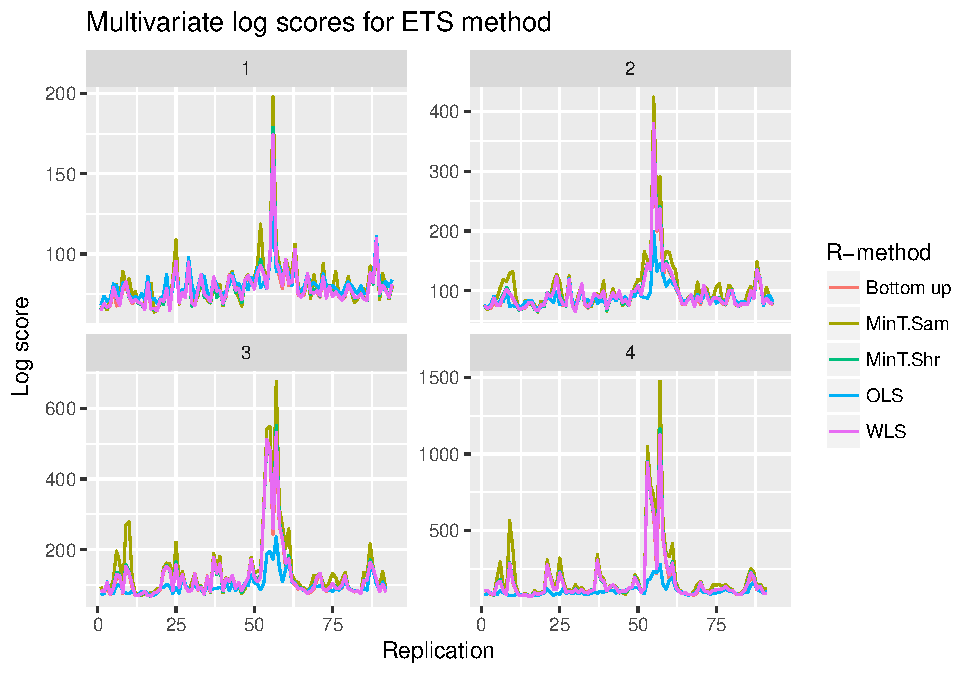
\includegraphics{Income-approach-results_files/figure-latex/unnamed-chunk-13-1.pdf}
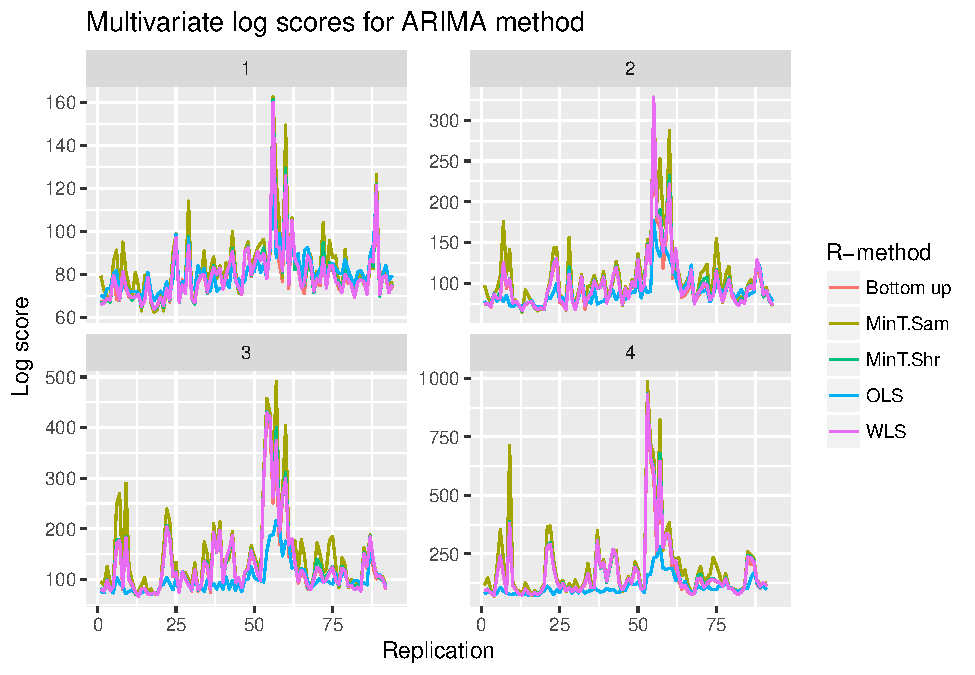
\includegraphics{Income-approach-results_files/figure-latex/unnamed-chunk-13-2.pdf}

\subsection{Predictive ability of univariate forecast
distributions}\label{predictive-ability-of-univariate-forecast-distributions-1}

\subsubsection{Summary of GDP - The most aggregate
series}\label{summary-of-gdp---the-most-aggregate-series-2}

\begin{table}[H]
\centering
\begin{tabular}{l|r|r|r|r|r|r|r|r|r|r|r|r|r|r|r|r}
\hline
\multicolumn{1}{c|}{ } & \multicolumn{8}{|c|}{ETS} & \multicolumn{8}{|c}{ARIMA} \\
\cline{2-9} \cline{10-17}
\multicolumn{1}{c|}{ } & \multicolumn{4}{|c|}{CRPS} & \multicolumn{4}{|c|}{LS} & \multicolumn{4}{|c|}{CRPS} & \multicolumn{4}{|c}{LS} \\
\cline{2-5} \cline{6-9} \cline{10-13} \cline{14-17}
Method & 1 & 2 & 3 & 4 & 1 & 2 & 3 & 4 & 1 & 2 & 3 & 4 & 1 & 2 & 3 & 4\\
\hline
Benchmark & -129.45 & -55.66 & -14.67 & -4.17 & -5.53 & 11.47 & 28.94 & 36.32 & -133.77 & -50.95 & -19.67 & -7.94 & -4.15 & 15.67 & 31.67 & 37.55\\
\hline
Base & 0.00 & 0.00 & 0.00 & 0.00 & 0.00 & 0.00 & 0.00 & 0.00 & 0.00 & 0.00 & 0.00 & 0.00 & 0.00 & 0.00 & 0.00 & 0.00\\
\hline
OLS & -0.82 & 1.61 & 2.64 & 1.09 & -1.27 & -1.57 & -1.10 & -1.18 & -0.25 & 1.11 & 0.15 & -0.06 & -0.73 & -1.07 & -1.37 & -1.82\\
\hline
WLS & -1.80 & 2.88 & 2.92 & -2.21 & -2.55 & -2.78 & -1.76 & -2.72 & -1.39 & 2.32 & 0.65 & -0.41 & -1.18 & -0.27 & 1.27 & 1.40\\
\hline
MinT Sample & 2.88 & 0.92 & -0.49 & -4.32 & -2.22 & -5.82 & -12.33 & -17.64 & -4.91 & -9.54 & -9.82 & -6.08 & -3.92 & -10.06 & -13.91 & -13.34\\
\hline
MinT Shrink & 1.01 & 4.31 & 3.22 & -1.83 & -1.95 & -2.81 & -3.96 & -6.27 & 0.89 & 1.17 & 0.43 & 0.78 & -1.11 & -1.45 & -1.69 & -1.87\\
\hline
\end{tabular}
\end{table}

\subsubsection{Summary of all aggregate level
series}\label{summary-of-all-aggregate-level-series-2}

\begin{table}[H]
\centering
\begin{tabular}{l|r|r|r|r|r|r|r|r|r|r|r|r|r|r|r|r}
\hline
\multicolumn{1}{c|}{ } & \multicolumn{8}{|c|}{ETS} & \multicolumn{8}{|c}{ARIMA} \\
\cline{2-9} \cline{10-17}
\multicolumn{1}{c|}{ } & \multicolumn{4}{|c|}{CRPS} & \multicolumn{4}{|c|}{LS} & \multicolumn{4}{|c|}{CRPS} & \multicolumn{4}{|c}{LS} \\
\cline{2-5} \cline{6-9} \cline{10-13} \cline{14-17}
Method & 1 & 2 & 3 & 4 & 1 & 2 & 3 & 4 & 1 & 2 & 3 & 4 & 1 & 2 & 3 & 4\\
\hline
Benchmark & -108.81 & -41.06 & -7.27 & 4.76 & -6.09 & 10.39 & 23.15 & 30.46 & -97.82 & -37.19 & -5.84 & 4.74 & -5.03 & 11.88 & 24.56 & 30.37\\
\hline
Base & 0.00 & 0.00 & 0.00 & 0.00 & 0.00 & 0.00 & 0.00 & 0.00 & 0.00 & 0.00 & 0.00 & 0.00 & 0.00 & 0.00 & 0.00 & 0.00\\
\hline
OLS & 1.43 & 1.86 & 1.48 & 1.33 & -1.12 & -2.70 & -4.01 & -4.50 & 1.29 & 1.27 & 0.53 & 1.15 & -1.21 & -2.91 & -4.50 & -5.15\\
\hline
WLS & 2.47 & 2.69 & 0.97 & -0.11 & -1.73 & -3.80 & -6.31 & -7.52 & 2.45 & 2.07 & 0.50 & 1.49 & -1.61 & -3.65 & -5.77 & -6.11\\
\hline
MinT Sample & 3.19 & -2.24 & -3.30 & -3.63 & -1.73 & -7.01 & -14.84 & -18.70 & -1.34 & -6.29 & -8.33 & -3.23 & -4.72 & -10.96 & -18.30 & -18.60\\
\hline
MinT Shrink & 4.02 & 3.13 & 1.40 & 0.59 & -1.52 & -4.22 & -8.03 & -9.58 & 5.22 & 2.49 & 0.51 & 3.26 & -1.61 & -4.40 & -8.44 & -8.88\\
\hline
\end{tabular}
\end{table}

\subsubsection{Summary of all disaggregate
series}\label{summary-of-all-disaggregate-series-2}

\begin{table}[H]
\centering
\begin{tabular}{l|r|r|r|r|r|r|r|r|r|r|r|r|r|r|r|r}
\hline
\multicolumn{1}{c|}{ } & \multicolumn{8}{|c|}{ETS} & \multicolumn{8}{|c}{ARIMA} \\
\cline{2-9} \cline{10-17}
\multicolumn{1}{c|}{ } & \multicolumn{4}{|c|}{CRPS} & \multicolumn{4}{|c|}{LS} & \multicolumn{4}{|c|}{CRPS} & \multicolumn{4}{|c}{LS} \\
\cline{2-5} \cline{6-9} \cline{10-13} \cline{14-17}
Method & 1 & 2 & 3 & 4 & 1 & 2 & 3 & 4 & 1 & 2 & 3 & 4 & 1 & 2 & 3 & 4\\
\hline
Benchmark & -74.79 & -29.85 & -4.80 & 5.13 & -8.12 & 9.06 & 28.41 & 43.29 & -72.44 & -28.79 & -4.24 & 4.85 & -7.85 & 10.01 & 29.56 & 44.08\\
\hline
Base & 0.00 & 0.00 & 0.00 & 0.00 & 0.00 & 0.00 & 0.00 & 0.00 & 0.00 & 0.00 & 0.00 & 0.00 & 0.00 & 0.00 & 0.00 & 0.00\\
\hline
OLS & -6.37 & -7.66 & -5.73 & -3.82 & -2.79 & 6.22 & 21.18 & 34.84 & -7.87 & -9.25 & -7.89 & -8.12 & -2.28 & 6.57 & 19.63 & 32.19\\
\hline
WLS & 1.64 & 0.61 & 0.28 & 0.20 & -0.13 & -0.84 & -1.07 & -0.90 & -0.31 & -0.35 & 0.24 & 0.26 & -0.25 & -0.94 & -1.05 & -1.15\\
\hline
MinT Sample & 0.72 & -3.14 & -2.34 & -4.16 & -1.65 & -5.48 & -8.13 & -10.65 & -6.11 & -8.48 & -9.33 & -6.84 & -3.54 & -7.92 & -10.66 & -10.88\\
\hline
MinT Shrink & 3.45 & 1.61 & 1.58 & 1.00 & 0.13 & -1.05 & -1.72 & -2.13 & 0.20 & -0.86 & -0.39 & 0.78 & -0.76 & -2.09 & -2.75 & -2.80\\
\hline
\end{tabular}
\end{table}

\subsubsection{Summary of all series in the
hierarchy}\label{summary-of-all-series-in-the-hierarchy-1}

\begin{table}[H]
\centering
\begin{tabular}{l|r|r|r|r|r|r|r|r|r|r|r|r|r|r|r|r}
\hline
\multicolumn{1}{c|}{ } & \multicolumn{8}{|c|}{ETS} & \multicolumn{8}{|c}{ARIMA} \\
\cline{2-9} \cline{10-17}
\multicolumn{1}{c|}{ } & \multicolumn{4}{|c|}{CRPS} & \multicolumn{4}{|c|}{LS} & \multicolumn{4}{|c|}{CRPS} & \multicolumn{4}{|c}{LS} \\
\cline{2-5} \cline{6-9} \cline{10-13} \cline{14-17}
Method & 1 & 2 & 3 & 4 & 1 & 2 & 3 & 4 & 1 & 2 & 3 & 4 & 1 & 2 & 3 & 4\\
\hline
Benchmark & -97.58 & -37.60 & -6.54 & 4.87 & -7.31 & 9.64 & 26.30 & 38.47 & -89.67 & -34.63 & -5.37 & 4.77 & -6.69 & 10.85 & 27.54 & 38.98\\
\hline
Base & 0.00 & 0.00 & 0.00 & 0.00 & 0.00 & 0.00 & 0.00 & 0.00 & 0.00 & 0.00 & 0.00 & 0.00 & 0.00 & 0.00 & 0.00 & 0.00\\
\hline
OLS & -1.15 & -1.08 & -0.65 & -0.17 & -2.09 & 2.41 & 10.97 & 20.04 & -1.65 & -1.94 & -1.95 & -1.54 & -1.73 & 2.47 & 9.79 & 18.27\\
\hline
WLS & 2.20 & 2.04 & 0.77 & -0.02 & -0.81 & -2.12 & -3.11 & -3.41 & 1.56 & 1.33 & 0.42 & 1.13 & -0.81 & -2.09 & -2.91 & -3.00\\
\hline
MinT Sample & 2.38 & -2.52 & -3.02 & -3.78 & -1.74 & -6.17 & -10.82 & -13.66 & -2.87 & -6.96 & -8.63 & -4.28 & -4.04 & -9.23 & -13.70 & -13.74\\
\hline
MinT Shrink & 3.83 & 2.66 & 1.46 & 0.71 & -0.58 & -2.41 & -4.20 & -4.96 & 3.60 & 1.47 & 0.24 & 2.54 & -1.04 & -3.04 & -5.05 & -5.05\\
\hline
\end{tabular}
\end{table}

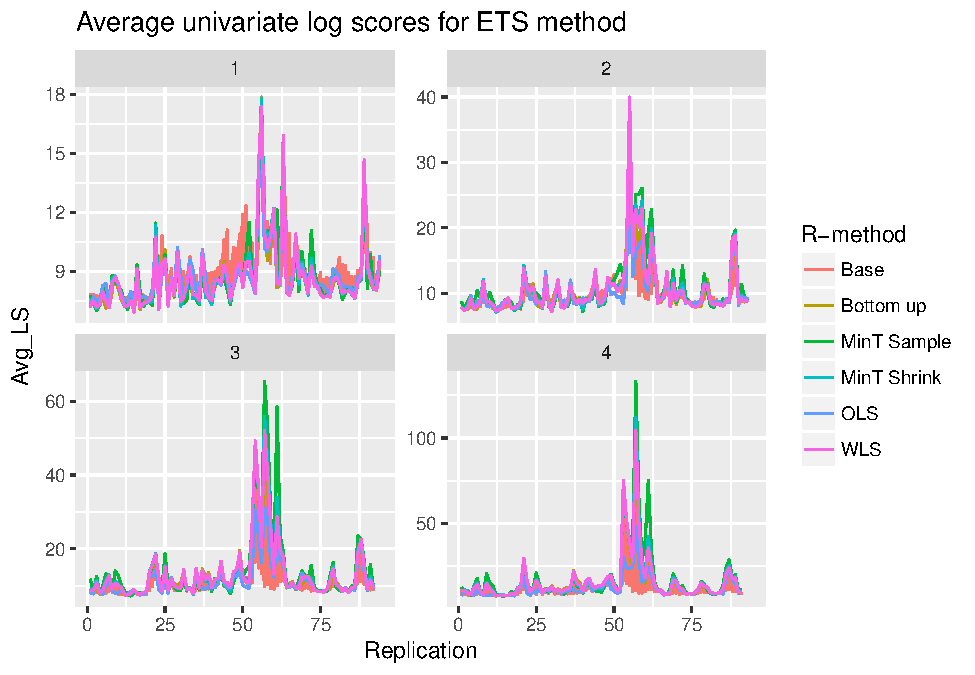
\includegraphics{Income-approach-results_files/figure-latex/unnamed-chunk-17-1.pdf}
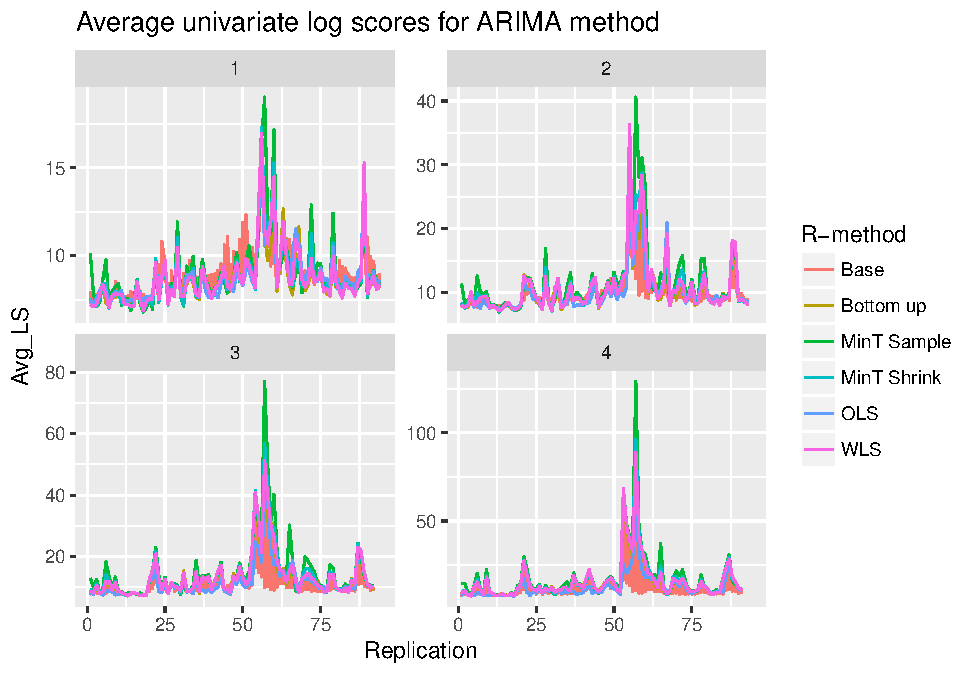
\includegraphics{Income-approach-results_files/figure-latex/unnamed-chunk-17-2.pdf}


\end{document}
